\section{Finite Element Method}

Many physical phenomena are described by partial differential equations (PDEs), but for anything but the simplest scenarios, these do not have an analytical closed-form solution; therefore numerical methods are needed for finding an approximate solution.
This is achieved by discretizing the problem, i.e. transforming a continuous problem into a discrete one.
There are numerous ways to discretize a problem, and some of the more popular schemes are finite difference (FDM), finite volume (FVM), and finite element method (FEM).\par

In this work we use FEM, which is a popular numerical scheme that offers some distinct advantages over other schemes for modeling VI.
FEM subdivides the domain of the PDE problem into many smaller subdomains called elements.
These elements can take a wide variety of shapes, e.g. tetrahedra, prisms, or cuboids for three-dimensional problems and triangles or rectangles for two-dimensional problems.
The collection of elements that make up the domain or geometry is called a \textit{mesh}.
The fineness of the mesh is what largely determines the accuracy of the solution, but also increases the computational costs.\par

The size of each element can be highly nonuniform which allows FEM to discretize complicated geometries.
This is advantageous for modeling VI, where different parts of the geometry can have dramatically different resolution requirements; the \SI{1}{\centi\metre} foundation crack requires elements on the scale of \si{\milli\metre}, while in other parts of the geometry the resolution requirement is on the scale of \si{\metre}.
This ability to easily represent complicated geometries with elements of non-uniform sizes helps maintain accuracy while saving computational resources.
Another benefit of using these elements is that it is easy to assign different constant values throughout the domain, and heterogenous materials can easily be represented.\par

The purpose of this work is not to provide a detailed description of the finite element method (FEM), but rather motivate the choice is using it over other numerical schemes and give some practical considerations of using it.
For the interested reader, there exists a wide body of work regarding FEM, and in this work \textit{The Finite Element Method: Theory, Implementation and Applications}\cite{larson_finite_2010} is continuously used as a source.\par

However, it is important to understand what determines the quality of the approximated solution.
For numerical schemes such as FDM, the quality of the solution is directly related to the fineness of the discretization (either in time or space).
While this is also true for FEM, there is another aspect that helps determine the quality of the approximated solution - the choice of \textit{basis function}.\par

Say that the function $u$ is the exact solution to some PDE in a given interval $I$, $u$ can then be approximated by $u_h$
\begin{equation}
  u \approx u_h
\end{equation}
where $u_h$ is a linear combination of basis functions and their respective \textit{nodal coefficients}.
\begin{equation}
  u_h = \sum^n_i u_i \psi_i \text{ in } I = [x_0, x_n], \; i = 0,\cdots,n
\end{equation}
$u_i$ is a nodal coefficient;
$\psi_i$ is a basis function;
where $x_0$ and $x_n$ are the end nodes of the interval $I$.\par

One of the key purposes of the basis functions is that they are used to transform a continuous PDE problem into a discrete one.
Exactly how this is achieved is not further described here, and the reader is referred to \textit{The Finite Element Method: Theory, Implementation and Applications}\cite{larson_finite_2010} for such details.
What matters is that the discretization results in a linear system of equations that may be solved to find all of the nodal coefficients $u_i$.
A wide variety of basis functions may be used, but simple ones are usually chosen, e.g. a "hat" functions or some lower-order polynomial, but it is not restricted to these.\par

An example of an approximation to some solution $u$ by $u_h$ as a linear combination of "hat" basis functions can be seen in Figure \ref{fig:approximate_solution}.
The combination basis functions $\psi_i$ with their respective nodal coefficients $u_i$ form $u_h$ which form a piecewise linear approximation of $u$.
This also shows why basis functions are often called \textit{interpolation functions} - they can be used to find the value of $u_h$ between nodes.
And just as when choosing functions for an interpolation scheme, i.e. whether to use piecewise linear or cubic splines, the choice of basis functions in FEM can affect the quality of the solution.\par

\begin{figure}[htb!]
  \centering
  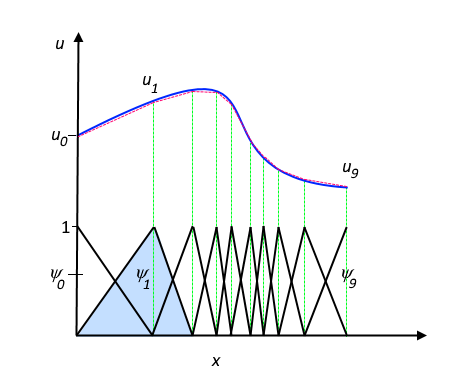
\includegraphics[width=0.75\textwidth]{approximate_solution.png}
  \caption[Basis functions are used to approximate the FEM solution to a PDE.]{The exact solution $u$ to some PDE (blue line) and its approximate solution $u_h$ (dashed red line). The "hat" basis functions $\psi_i$ (black lines) for each element of the interval. The combination of the each nodal coefficient $u_i$ and basis function $\psi_i$ form the piecewise linear approximation $u_h$ of $u$. Figure from COMSOL\cite{noauthor_detailed_nodate}.}
  \label{fig:approximate_solution}
\end{figure}

Using a higher-order basis functions can be much more computationally expensive, and thus typically simple ones are favored - such as hat functions or second order polynomials.
The fineness of the mesh becomes more important with simpler basis functions, and becomes the primary means for improving the solution quality.
However, there are circumstances when increasing mesh fineness is impossible, and in such cases choosing a higher-order basis function may improve the quality instead.\par

In this work we use a commercial FEM software called COMSOL Multiphysics, where subsequent sections will cover the steps required to implement our VI model in COMSOL.
(Of course, this could easily be translated into use in another software package.)\par

In order, we will cover:
\begin{enumerate}
  \item Creation of a model geometry.
  \item Defining physics/governing equations, boundary, and initial conditions.
  \item Discretize/mesh the geometry.
  \item Solver configuration.
  \item Post-process the results.
\end{enumerate}
